\section{AgentRole}
\label{sec:AgentRole}
%%%%%%%%%%%%%%%%%%%%%%%%%%%%%%%%%%%%%%%%%%%%%%%%%%%%%%%%
\begin{figure}[h!]
\begin{center}
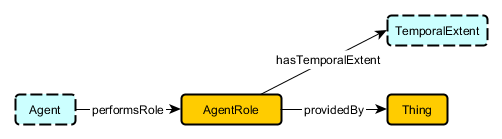
\includegraphics[width=.8\textwidth]{figures/agentrole}
\end{center}
\caption{Schema Diagram for the AgentRole Pattern. The visual notation is explained in Chapter \ref{chap:prelims}.}
\label{fig:AgentRole}
\end{figure}
\subsection{Summary}
\label{sum:AgentRole}
%%%%%%%%%%%%%%%%%%%%%%%%%%%%
The \textsf{AgentRole} pattern is essentially a reification of association with something. That is, it's very unlikely that an Agent will be associated with something for all time. Thus, the association relation is not binary, perhaps $\textit{associated}(x,y,t)$, agent $x$ is associated with thing $y$ at time $t$. Thus, the reification. The association becomes a concept in its own right and has a temporal extent, allowing an \textsf{Agent} to be associated to a \textsf{Thing} (e.g. \textsf{Event}, Section \ref{sec:Event}) for some \textsf{TemporalExtent}. 

%%%%%%%%%%%%%%%%%%%%%%%%%%%%%%%%%%%%%%%%%%%%%%%%%%%%%%%%
\subsection{Axiomatization}
\label{axs:AgentRole}
%%%%%%%%%%%%%%%%%%%%%%%%%%%%
\begin{align}
% General
\textsf{AgentRole} &\sqsubseteq \text{=1}\textsf{isPerformedBy.Agent} \\
\textsf{AgentRole} &\sqsubseteq \text{=1}\textsf{hasTemporalExtent.TemporalExtent} \\
% Domain and Range Restrictions
\exists\textsf{isPerformedBy.Agent} &\sqsubseteq \textsf{AgentRole} \\
\textsf{AgentRole} &\sqsubseteq \forall\textsf{isPerformedBy.Agent} \\
\exists\textsf{hasTemporalExtent.TemporalExtent} &\sqsubseteq \textsf{AgentRole} \\
\top &\sqsubseteq \forall\textsf{hasTemporalExtent.TemporalExtent} \\
\top &\sqsubseteq \forall\textsf{providesAgentRole.AgentRole} \\
% Inverses
\textsf{isPerformedBy} &\equiv \textsf{performsAgentRole}^- \\
\textsf{isProvidedBy} &\equiv \textsf{providesAgentRole}^-
\end{align}

%%%%%%%%%%%%%%%%%%%%%%%%%%%%%%%%%%%%%%%%%%%%%%%%%%%%%%%%
\subsection{Explanations}
\label{exp:AgentRole}
%%%%%%%%%%%%%%%%%%%%%%%%%%%%
\begin{enumerate}
\item Exactly one \textsf{Agent} performs an \textsf{AgentRole}.
\item An \textsf{AgentRole} has exactly one \textsf{TemporalExtent}.
\item Scoped Domain: the scoped domain of \textsf{isPerformedBy}, scoped by \textsf{Agent}, is \textsf{AgentRole}.
\item Scoped Range: the scoped range of \textsf{isPerformedBy}, scoped by \textsf{AgentRole}, is \textsf{Agent}. 
\item Scoped Domain: the scoped domain of \textsf{hasTemporalExtent}, scoped by \textsf{TemporalExtent}, is \textsf{AgentRole}.
\item Range: the range of \textsf{hasTemporalExtent} is \textsf{TemporalExtent}.
\item Range:  the range of \textsf{providesAgentRole} is \textsf{AgentRole}.
\item Inverse Alias.
\item Inverse Alias.
\end{enumerate}

%%%%%%%%%%%%%%%%%%%%%%%%%%%%%%%%%%%%%%%%%%%%%%%%%%%%%%%%
\subsection{Competency Questions}
\label{cqs:AgentRole}
%%%%%%%%%%%%%%%%%%%%%%%%%%%%
\begin{enumerate}[CQ1.]
\item When was Cogan Shimizu a student at Wright State University?
\item Who was the lead actor for the movie, Sharknado?
\item Who was on the World Cup winning team in 2017?
\end{enumerate}

\newpage
%%%%%%%%%%%%%%%%%%%%%%%%%%%%%%%%%%%%%%%%%%%%%%%%%%%%%%%%
% End Section
%%%%%%%%%%%%%%%%%%%%%%%%%%%%%%%%%%%%%%%%%%%%%%%%%%%%%%%%
%%%%%%%%%%%%%%%%%%%%%%%%%%%%%%%%%%%%%%%%%%%%%%%%%%%%%%%%